\setcounter{section}{8}
\section{Methode der Kleinsten Quadrate und QR-Zerlegung}

\subsection{Methode der kleinsten Quadrate}

Die Methode der kleinsten Quadrate wird immer dann angewendet, wenn wir eine möglichst \textit{gute} Lösung für ein überbestimmtes Gleichungssystem \( Ax = c\) finden wollen, für welches es keine eindeutige Lösung gibt. Ein Gleichungssystem ist überbestimmt, wenn es mehr Gleichungen als Unbekannte hat. Für die Matrix \( A \in \mathbb{R}^{m \times n} \) gilt dann \(m > n \). In realen Anwendungen sind Gleichungssysteme sehr oft Überbestimmt, weswegen es wichtig ist für solche Systeme möglichst \textit{gute} Lösungen zu finden. Was dabei eine \textit{gute} Lösung ausmacht, betrachten wir im folgenden Beispiel. 

\vspace{1\baselineskip}

Bei einer Umfrage werden Menschen bezüglich Körpergrösse und Schuhgrösse befragt. Wir wollen einen Zusammenhang zwischen Körpergrösse und Schuhgrösse finden damit wir nachher basierend auf der Schuhgrösse eine Schätzung für die Körpergrösse machen können. Wir suchen also eine Gleichung der Form

\begin{figure*}[h]
    \centering
    \begin{minipage}
        {0.5\textwidth}
        \begin{equation*}
            \text{Körpergrösse} = x_1\cdot \text{Schuhgrösse} + x_2, \quad (\ddagger)
        \end{equation*}        
    \end{minipage}
    \hfill
    \begin{minipage}
        {0.45\textwidth}
        \centering
        \tikzsetnextfilename{kleinste_quadrate_schuhe_01}
        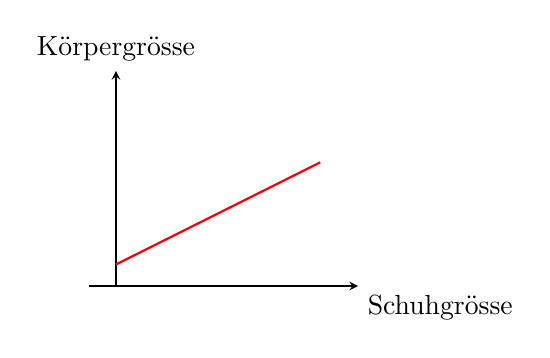
\begin{tikzpicture}
            \begin{axis}[
                width = 5cm,
                axis lines = middle,
                xlabel = {\text{Schuhgrösse}},
                ylabel = {\text{Körpergrösse}},
                xlabel style={below right},
                ylabel style={above}, 
                xmin=0, xmax=10,
                ymin=0, ymax=10,
                axis equal,
                xtick=\empty,
                ytick=\empty,
            ]
            \addplot [
                domain=0:9.5, 
                samples=5, 
                color=red,
                thick, 
            ]
            { 0.5*x +1 };
            % \node[pin={[pin edge={<-, thick, black}]right:{\( b \)}}] at (axis cs:0,1,0) {};
            \end{axis}
        \end{tikzpicture}
    \end{minipage}
\end{figure*}
    


wobei die Koeffizienten \( x_1, x_2\) unbekannt sind und experimentell durch eine Umfrage ermittelt werden. In einer Umfrage werden nun 8 Menschen befragt, wodurch wir für zwei Unbekannte \( x_1\) und \( x_2\), 8 Gleichungen erhalten. Wir werden also keine eindeutige Lösung für \( x_1\) und \( x_2\) finden können. Wie wählen wir nun die besten Werte für \( x_1\) und \( x_2\) damit die Gleichung \( (\ddagger) \) möglichst gut die Realität repräsentiert? Betrachten wir zunächst die Werte der Umfrage. Aus einer Tabelle mit allen Umfragewerten können wir das überstimmte LGS \( Ax = c \) aufstellen. 

\vspace{1\baselineskip}

\begin{minipage}
    {0.5\textwidth}
    \centering
        \begin{tabular}{|c|c|}
            \hline
            Schuhgrösse & Körpergrösse \\
            \hline
            41 & 172 \\
            45 & 190 \\
            42 & 180 \\
            43 & 183 \\
            43 & 178 \\
            38 & 163 \\
            44 & 180 \\
            40 & 178 \\
            \hline
        \end{tabular}
\end{minipage}
\hfill
\begin{minipage}
    {0.45\textwidth}
    \centering
    \begin{equation*}
        \begin{aligned}
            172 &= x_1\cdot 41 + x_2\\
            190 &= x_1\cdot 45 + x_2\\
            180 &= x_1\cdot 42 + x_2\\
            183 &= x_1\cdot 43 + x_2\\
            178 &= x_1\cdot 43 + x_2\\
            163 &= x_1\cdot 38 + x_2\\
            180 &= x_1\cdot 44 + x_2\\
            178 &= x_1\cdot 40 + x_2\\
        \end{aligned}
    \end{equation*}
\end{minipage}

\vspace{1\baselineskip}

Die Matrix \( A \in \mathbb{R}^{8 \times 2} \) und der Vektor \( c \in \mathbb{R}^{8 \times 1} \) sind dann wie folgt definiert:

\begin{equation*}
    A = \begin{pmatrix}
        41 & 1 \\
        45 & 1 \\
        \vdots & \vdots \\
        40 & 1 \\
    \end{pmatrix}, \quad
    c = \begin{pmatrix}
        172 \\ 190 \\ \vdots \\ 178
    \end{pmatrix}.
\end{equation*}


\vspace{1\baselineskip}

Wir können nun alle Messwerte in einem Koordinatensystem auftragen um zu sehen, wie der Zusammenhang zwischen Schuhgrösse und Körpergrösse aussieht. Als Nächstes wollen wir eine Gerade der Form~\( (\ddagger) \) finden, die möglichst nah an allen Messpunkten ist. Ein Weg dies zu erreichen ist es alle Abstände \( r_i \) von der Geraden zu den Messwerten zu minimieren. 

\vspace{1\baselineskip}

\begin{figure*}[h]
    \centering
    \begin{minipage}
        {0.7\textwidth}
        \centering
        \tikzsetnextfilename{kleinste_quadrate_schuhe_02}
        \begin{tikzpicture}
            \begin{axis}[
                width = 8cm,
                axis lines = middle,
                xlabel = {\text{Schuhgrösse}},
                ylabel = {\text{Körpergrösse}},
                xlabel style={below right},
                ylabel style={above}, 
                xmin=37, xmax=47,
                ymin=155, ymax=195,
            ]
                \addplot[
                    only marks,
                    mark=*,
                    color=black
                ] coordinates {
                    (41,172)
                    (45,190)
                    (42,180)
                    (43,183)
                    (43,178)
                    (38,163)    
                    (44,180)
                    (40,178)
                };
                \addplot[
                    domain=37:46, 
                    samples=5, 
                    color=red,
                    thick, 
                    dotted,
                    opacity =0.5,
                ]
                { 3.083*x +48.5 };
                \addplot[
                    color=orange, 
                    thick       
                ] coordinates {
                    (40,178)   
                    (40, 3.083*40 +48.5 )   
                };
                \addplot[
                    color=orange, 
                    thick       
                ] coordinates {
                    (41,172)   
                    (41, 3.083*41 +48.5 )   
                };
                \addplot[
                    color=orange, 
                    thick       
                ] coordinates {
                    (42,180)   
                    (42, 3.083*42 +48.5 )   
                };
                \addplot[
                    color=orange, 
                    thick       
                ] coordinates {
                    (43,183)   
                    (43, 3.083*43 +48.5 )   
                };
                \addplot[
                    color=orange, 
                    thick       
                ] coordinates {
                    (43,178)   
                    (43, 3.083*43 +48.5 )   
                };
                \addplot[
                    color=orange, 
                    thick       
                ] coordinates {
                    (38,163)   
                    (38, 3.083*38 +48.5 )   
                };
                \addplot[
                    color=orange, 
                    thick       
                ] coordinates {
                    (44,180)   
                    (44, 3.083*44 +48.5 )   
                };
                \addplot[
                    color=orange, 
                    thick       
                ] coordinates {
                    (45,190)   
                    (45, 3.083*45 +48.5 )   
                };
                \node[pin={[pin edge={<-, thick, black}]left:{\( r_i \)}}] at (axis cs:40,175,0) {};
            \end{axis}
        \end{tikzpicture}
    \end{minipage}    
    \hfill
    \begin{minipage}
        {0.29\textwidth}
        \centering
        \begin{equation*}
            \begin{aligned}
                r_1 &= (x_1\cdot 41 + x_2) - 172 \\
                r_2 &= (x_1\cdot 45 + x_2) - 190 \\
                r_3 &= (x_1\cdot 42 + x_2) - 180 \\
                r_4 &= (x_1\cdot 43 + x_2) - 183 \\
                r_5 &= (x_1\cdot 43 + x_2) - 178 \\
                r_6 &= (x_1\cdot 38 + x_2) - 163 \\
                r_7 &= (x_1\cdot 44 + x_2) - 180 \\
                r_8 &= (x_1\cdot 40 + x_2) - 178 \\
            \end{aligned}
        \end{equation*}
    \end{minipage}
\end{figure*}

Da alle Abstände gleichzeitig minimiert werden sollen, fassen wir alle \( r_i \) im sogenannten Residuenvektor \( r = (r_1, \dots, r_m)^\top \) zusammen und minimieren dann die gesamte Länge von \( r \), das entspricht der quadratischen Minimierung des Fehlers \( r \). Wir suchen also das \( x \) sodass

\begin{equation*}
    \lVert r \rVert_2 = \lVert A x - c \rVert_2,
\end{equation*}

\vspace{0.25\baselineskip}

minimal wird. In unserem Fall suchen wir \( x^{opt} = (x_1^{opt} \ \ \ x_2^{opt})^\top\) welches die Länge von \( r \) minimiert. Aber wie können wir dieses Problem lösen? Betrachten wir dafür ein reduziertes Gleichungssystem mit nur drei Gleichungen und zwei Unbekannten, dafür nehmen wir einfach die ersten drei Messwerte von oben. 

\begin{equation*}
    \begin{aligned}
        x_1\cdot 41 + x_2&= 172 \\
        x_1\cdot 45 + x_2&= 190 \\
        x_1\cdot 42 + x_2&= 180 \\
    \end{aligned} \qquad \rightarrow \qquad
    \begin{aligned}
        \underbrace{
        \begin{pmatrix}
            41 & 1 \\
            45 & 1 \\
            42 & 1 \\
        \end{pmatrix}}_{A}
        \begin{pmatrix}
            x_1\\ x_2
        \end{pmatrix}
        =
        \underbrace{
        \begin{pmatrix}
            172 \\ 190 \\ 180
        \end{pmatrix}}_{c} \\
    \end{aligned}
\end{equation*}

Genau wie oben ist dieses LGS überbestimmt und in dieser Form nicht exakt lösbar. Grafisch können wir uns das Problem wie folgt vorstellen. 

\newpage

\begin{figure*}[h]
    \centering
    \tikzsetnextfilename{kleinste_quadrate_schuhe_03}
    \begin{tikzpicture}[x=0.75pt,y=0.75pt,yscale=-1,xscale=1]
        %uncomment if require: \path (0,387); %set diagram left start at 0, and has height of 387
        %Straight Lines [id:da7205339018057622] 
        \draw    (200,280) -- (200,23) ;
        \draw [shift={(200,20)}, rotate = 90] [fill={rgb, 255:red, 0; green, 0; blue, 0 }  ][line width=0.08]  [draw opacity=0] (5.36,-2.57) -- (0,0) -- (5.36,2.57) -- (3.56,0) -- cycle    ;
        %Straight Lines [id:da2519180835664382] 
        \draw    (170,160) -- (347.5,278.34) ;
        \draw [shift={(350,280)}, rotate = 213.69] [fill={rgb, 255:red, 0; green, 0; blue, 0 }  ][line width=0.08]  [draw opacity=0] (5.36,-2.57) -- (0,0) -- (5.36,2.57) -- (3.56,0) -- cycle    ;
        %Straight Lines [id:da9037439858367798] 
        \draw    (170,190) -- (407.15,110.95) ;
        \draw [shift={(410,110)}, rotate = 161.57] [fill={rgb, 255:red, 0; green, 0; blue, 0 }  ][line width=0.08]  [draw opacity=0] (5.36,-2.57) -- (0,0) -- (5.36,2.57) -- (3.56,0) -- cycle    ;
        %Straight Lines [id:da43986582741717895] 
        \draw [color={rgb, 255:red, 126; green, 211; blue, 33 }  ,draw opacity=1 ][line width=1.5]    (200,180) -- (306.14,208.95) ;
        \draw [shift={(310,210)}, rotate = 195.26] [fill={rgb, 255:red, 126; green, 211; blue, 33 }  ,fill opacity=1 ][line width=0.08]  [draw opacity=0] (6.43,-3.09) -- (0,0) -- (6.43,3.09) -- (4.27,0) -- cycle    ;
        %Straight Lines [id:da8398239923702847] 
        \draw [color={rgb, 255:red, 126; green, 211; blue, 33 }  ,draw opacity=1 ][line width=1.5]    (200,180) -- (256.93,132.56) ;
        \draw [shift={(260,130)}, rotate = 140.19] [fill={rgb, 255:red, 126; green, 211; blue, 33 }  ,fill opacity=1 ][line width=0.08]  [draw opacity=0] (6.43,-3.09) -- (0,0) -- (6.43,3.09) -- (4.27,0) -- cycle    ;
        %Shape: Polygon [id:ds9350103434885011] 
        \draw  [color={rgb, 255:red, 126; green, 211; blue, 33 }  ,draw opacity=0.75 ][fill={rgb, 255:red, 126; green, 211; blue, 33 }  ,fill opacity=0.25 ][dash pattern={on 4.5pt off 4.5pt}] (260,130) -- (200,180) -- (310,210) -- (370,160) -- (370,160) -- cycle ;
        % %Curve Lines [id:da7687484645278241] 
        % \draw [color={rgb, 255:red, 126; green, 211; blue, 33 }  ,draw opacity=1 ]   (380,170) .. controls (359.31,185.8) and (354.46,179.81) .. (351.17,172.66) ;
        % \draw [shift={(350,170)}, rotate = 66.37] [fill={rgb, 255:red, 126; green, 211; blue, 33 }  ,fill opacity=1 ][line width=0.08]  [draw opacity=0] (5.36,-2.57) -- (0,0) -- (5.36,2.57) -- (3.56,0) -- cycle    ;
        %Straight Lines [id:da14079628618044737] 
        \draw [color={rgb, 255:red, 208; green, 2; blue, 27 }  ,draw opacity=1 ][line width=1.5]    (200,180) -- (316.05,160.66) ;
        \draw [shift={(320,160)}, rotate = 170.54] [fill={rgb, 255:red, 208; green, 2; blue, 27 }  ,fill opacity=1 ][line width=0.08]  [draw opacity=0] (6.43,-3.09) -- (0,0) -- (6.43,3.09) -- (4.27,0) -- cycle    ;
        %Straight Lines [id:da38161966038314155] 
        \draw [color={rgb, 255:red, 74; green, 144; blue, 226 }  ,draw opacity=1 ][line width=1.5]    (200,180) -- (316.67,102.22) ;
        \draw [shift={(320,100)}, rotate = 146.31] [fill={rgb, 255:red, 74; green, 144; blue, 226 }  ,fill opacity=1 ][line width=0.08]  [draw opacity=0] (6.43,-3.09) -- (0,0) -- (6.43,3.09) -- (4.27,0) -- cycle    ;
        %Straight Lines [id:da5231184422285943] 
        \draw [color={rgb, 255:red, 245; green, 166; blue, 35 }  ,draw opacity=1 ][line width=1.5]    (320,100) -- (320,156) ;
        \draw [shift={(320,160)}, rotate = 270] [fill={rgb, 255:red, 245; green, 166; blue, 35 }  ,fill opacity=1 ][line width=0.08]  [draw opacity=0] (6.43,-3.09) -- (0,0) -- (6.43,3.09) -- (4.27,0) -- cycle    ;
        %Curve Lines [id:da3839403950250917] 
        \draw [color={rgb, 255:red, 0; green, 0; blue, 0 }  ,draw opacity=1 ]   (360,200) .. controls (333.25,201.94) and (311.79,191.65) .. (291.85,171.86) ;
        \draw [shift={(290,170)}, rotate = 45.69] [fill={rgb, 255:red, 0; green, 0; blue, 0 }  ,fill opacity=1 ][line width=0.08]  [draw opacity=0] (5.36,-2.57) -- (0,0) -- (5.36,2.57) -- (3.56,0) -- cycle    ;
        %Curve Lines [id:da9653910687163929] 
        \draw [color={rgb, 255:red, 0; green, 0; blue, 0 }  ,draw opacity=1 ]   (300,60) .. controls (292.84,78.62) and (289.32,91.32) .. (298.6,107.66) ;
        \draw [shift={(300,110)}, rotate = 237.85] [fill={rgb, 255:red, 0; green, 0; blue, 0 }  ,fill opacity=1 ][line width=0.08]  [draw opacity=0] (5.36,-2.57) -- (0,0) -- (5.36,2.57) -- (3.56,0) -- cycle    ;
        %Curve Lines [id:da8838459359016881] 
        \draw [color={rgb, 255:red, 0; green, 0; blue, 0 }  ,draw opacity=1 ]   (370,90) .. controls (347.44,94.32) and (351.61,115.69) .. (328.97,119.6) ;
        \draw [shift={(326,120)}, rotate = 354.51] [fill={rgb, 255:red, 0; green, 0; blue, 0 }  ,fill opacity=1 ][line width=0.08]  [draw opacity=0] (5.36,-2.57) -- (0,0) -- (5.36,2.57) -- (3.56,0) -- cycle    ;
        % % Text Node
        % \draw (381,161) node [anchor=north west][inner sep=0.75pt]  [color={rgb, 255:red, 126; green, 211; blue, 33 }  ,opacity=1 ] [align=left] {Bild von \( A \)};
        % Text Node
        \draw (309,213) node [anchor=north west][inner sep=0.75pt]  [color={rgb, 255:red, 126; green, 211; blue, 33 }  ,opacity=1 ] [align=left] {\( a^{(1)} \)};
        % Text Node
        \draw (223,112) node [anchor=north west][inner sep=0.75pt]  [color={rgb, 255:red, 126; green, 211; blue, 33 }  ,opacity=1 ] [align=left] {\( a^{(2)} \)};
        % Text Node
        \draw (365,200) node [anchor=west][inner sep=0.75pt]  [color={rgb, 255:red, 0; green, 0; blue, 0 }  ,opacity=1 ] [align=left] {\( A \textcolor{customred}{x^{opt}} \in \textcolor{customgreen}{\text{Bild}A} \) };
        % Text Node
        \draw (270,42) node [anchor=north west][inner sep=0.75pt]  [color={rgb, 255:red, 0; green, 0; blue, 0 }  ,opacity=1 ] [align=left] {\( \textcolor{customblue}{c} \notin \textcolor{customgreen}{\text{Bild}A} \)};
        % Text Node
        \draw (375,90) node [anchor=west][inner sep=0.75pt]  [color={rgb, 255:red, 0; green, 0; blue, 0 }  ,opacity=1 ] [align=left] {\( \textcolor{customorange}{r} =  A \textcolor{customred}{x^{opt}} - \textcolor{customblue}{c} \)};
        % Text Node
        \draw (200,282) node [anchor=north][inner sep=0.75pt]  [font=\scriptsize,color={rgb, 255:red, 0; green, 0; blue, 0 }  ,opacity=1 ] [align=center] {nicht Massstäblich};
    \end{tikzpicture}
\end{figure*}

Der Vektor \( x^{opt} \) repräsentiert hier die optimale Lösung, welche den kürzesten Residuenvektor \( r \) hat und im Bild von \( A \) liegt. Grafisch können wir hier auch sehen, dass der Vektor \( r \) minimal ist, wenn er orthogonal zum \( \text{Bild}A \) ist. Für die optimale Lösung muss also gelten:

\begin{equation*}
    \underbrace{A y}_{\text{Bild}A} \ \perp \ r \ , \quad \forall y \in \mathbb{R}^n.
\end{equation*}

Mit dem Skalarprodukt können wir das umformulieren zu

\begin{equation*}
    \langle A  y, r \rangle = 0,
\end{equation*}

\begin{equation*}
    (A  y)^\top  r = 0.
\end{equation*}

Nun können wir unsere Definition für \( r \) einsetzen

\begin{equation*}
    y^\top A^\top \left( A x^{opt} -c \right) = 0, 
\end{equation*}

und alles ausmultiplizieren

\begin{equation*}
    y^\top A^\top A x^{opt} - y^\top A^\top c  = 0.
\end{equation*}

Schliesslich können wir noch umstellen und nach \( x^{opt} \) auflösen

\begin{equation*}
    A^\top c = A^\top A x^{opt},
\end{equation*}

\begin{equation*}
    (A^\top A)^{-1} A^\top c = x^{opt}.
\end{equation*}

Dieser Ausdruck gibt uns nun die optimale Lösung, indem der quadratische Fehler (Länge des Residuenvektors) minimiert wird. Oft wollen wir jedoch nicht die inverse von \( A^\top A \) berechnen und können alternativ das folgende LGS lösen

\begin{equation*}
    A^\top A x^{opt} = A^\top c.
\end{equation*}

\begin{tcolorbox}[colback=gray!30, colframe=gray!80, title=Kleinste Quadrate]
    Wir wollen die optimale Lösung \( x^{opt} \) finden welche den quadratischen Fehler \( \lVert r \rVert_2 = \lVert A x - c \rVert_2 \) minimiert. Oft ist das LGS schon in der Form \( Ax - c = r \) gegeben. 
    \begin{enumerate}
        \item Bestimme \( A \) und \( c \)
        \item Berechne \( A^\top A \) und \( A^\top c \)
        \item Löse das LGS \( A^\top A x^{opt} = A^\top c \)
    \end{enumerate}
\end{tcolorbox}

\subsection{QR-Zerlegung}

Bei der QR-Zerlegung werden wir eine Matrix \( A \in \mathbb{R}^{m \times n} \) in das Produkt einer orthogonalen Matrix \( Q \in \mathbb{R}^{m \times m} \) und einer oberen Dreiecksmatrix \( R \in \mathbb{R}^{m \times n} \) zerlegen. Es gilt dann 

\vspace{1\baselineskip}

\begin{figure}[h]
    \tikzsetnextfilename{qr_zerlegung_01}
    \centering
    \begin{tikzpicture}[x=0.75pt,y=0.75pt,yscale=-1,xscale=1]
        %uncomment if require: \path (0,300); %set diagram left start at 0, and has height of 300
        
        %Shape: Rectangle [id:dp842902263884775] 
        \draw   (170,50) -- (230,50) -- (230,140) -- (170,140) -- cycle ;
        %Shape: Rectangle [id:dp1365802461569866] 
        \draw   (300,50) -- (390,50) -- (390,140) -- (300,140) -- cycle ;
        %Shape: Rectangle [id:dp06826642370754088] 
        \draw   (440,50) -- (500,50) -- (500,140) -- (440,140) -- cycle ;
        %Straight Lines [id:da11387891999511401] 
        \draw  [dash pattern={on 4.5pt off 4.5pt}]  (450,60) -- (490,100) ;
        
        % Text Node
        \draw (141,90) node [anchor=north west][inner sep=0.75pt]   [align=left] {$\displaystyle m$};
        % Text Node
        \draw (191,147) node [anchor=north west][inner sep=0.75pt]   [align=left] {$\displaystyle n$};
        % Text Node
        \draw (241,90) node [anchor=north west][inner sep=0.75pt]   [align=left] {$\displaystyle =$};
        % Text Node
        \draw (271,90) node [anchor=north west][inner sep=0.75pt]   [align=left] {$\displaystyle m$};
        % Text Node
        \draw (341,147) node [anchor=north west][inner sep=0.75pt]   [align=left] {$\displaystyle m$};
        % Text Node
        \draw (401,90) node [anchor=north west][inner sep=0.75pt]   [align=left] {$\displaystyle \cdot $};
        % Text Node
        \draw (191,12) node [anchor=north west][inner sep=0.75pt]   [align=left] {$\displaystyle A$};
        % Text Node
        \draw (341,12) node [anchor=north west][inner sep=0.75pt]   [align=left] {$\displaystyle Q$};
        % Text Node
        \draw (411,90) node [anchor=north west][inner sep=0.75pt]   [align=left] {$\displaystyle m$};
        % Text Node
        \draw (461,147) node [anchor=north west][inner sep=0.75pt]   [align=left] {$\displaystyle n$};
        % Text Node
        \draw (461,12) node [anchor=north west][inner sep=0.75pt]   [align=left] {$\displaystyle R$};
        % Text Node
        \draw (241,16) node [anchor=north west][inner sep=0.75pt]   [align=left] {$\displaystyle =$};
        % Text Node
        \draw (401,16) node [anchor=north west][inner sep=0.75pt]   [align=left] {$\displaystyle \cdot $};
        % Text Node
        \draw (451,90) node [anchor=north west][inner sep=0.75pt]   [align=left] {$\displaystyle 0$};
        % Text Node
        \draw (481,118) node [anchor=north west][inner sep=0.75pt]   [align=left] {$\displaystyle 0$};
        % Text Node
        \draw (451,118) node [anchor=north west][inner sep=0.75pt]   [align=left] {$\displaystyle 0$};
    \end{tikzpicture}
\end{figure}    

Später können wir die QR-Zerlegung als ein alternatives Lösungsverfahren der kleinsten Quadrate verwenden. Um die QR-Zerlegung zu berechnen, müssen einige Schritte befolgt werden. Betrachten wir das Ganze an einem Beispiel.

\vspace{1\baselineskip}

Wir suchen nun \( Q \) und \( R \) sodass für die Matrix 

\begin{equation*}
    A = \begin{pmatrix}
        1 & 0 \\
        0 & 1 \\
        1 & 1 \\
    \end{pmatrix},
\end{equation*}

gilt \( A = QR \). Dafür eliminieren wir schrittweise alle Elemente \( a_{ij} \) unterhalb der Hauptdiagonalen von \( A \). In unserem fall beginnen wir mit dem Eintrag \( a_{31} \). Zuerst notieren wir die Werte für \( i, j \) und die Einträge \( a_{jj}, \ a_{ij} \) 

\begin{equation*}
    i = 3, \ j = 1. 
\end{equation*}

\begin{equation*}
    a_{jj} = 1, \ a_{ij} = 1.
\end{equation*}

Anschliessend berechnen wir den Wert einer Zwischenvariable \( \omega \) gegeben durch

\begin{equation*}
    \omega = \sqrt{a_{jj}^2 + a_{ij}^2} = \sqrt{1^2 + 1^2} = \sqrt{2}.
\end{equation*}

Als Nächstes suchen wir eine Rotationsmatrix \( Q^{\prime \top} \). Dafür fangen wir mit einer Identitätsmatrix \( I \in \mathbb{R}^{m \times m} \) an und füllen die Einträge wie folgt ein

\begin{equation*}
    i_{ii} = \cos(\alpha), \ i_{ij} = -\sin(\alpha), \ i_{ji} = \sin(\alpha), \ i_{jj} = \cos(\alpha).
\end{equation*}

Wobei die spezifischen Werte für cos und sin durch das \( \omega \) gegeben sind

\begin{equation*}
    \sin(\alpha) = \frac{a_{ij}}{\omega} = \frac{1}{\sqrt{2}}, \quad \cos(\alpha) = \frac{a_{jj}}{\omega} = \frac{1}{\sqrt{2}}.
\end{equation*}

In unserem Fall ist \( Q'^\top \) gegeben durch

\begin{equation*}
    Q'^\top = \begin{pmatrix}
        \cos(\alpha) & 0 & \sin(\alpha) \\
        0 & 1 & 0 \\
        - \sin(\alpha) & 0 & \cos(\alpha) \\
    \end{pmatrix} =
    \begin{pmatrix}
        \frac{1}{\sqrt{2}} & 0 & \frac{1}{\sqrt{2}} \\
        0 & 1 & 0 \\
        -\frac{1}{\sqrt{2}} & 0 & \frac{1}{\sqrt{2}} \\
    \end{pmatrix}.
\end{equation*}

Nun Berechnen wir die Matrix \( A' = Q'^\top A \) und überprüfen ob \( A' \) eine obere Dreiecksmatrix ist.

\begin{equation*}
    A' = Q'^\top A = 
    \begin{pmatrix}
        \frac{1}{\sqrt{2}} & 0 & \frac{1}{\sqrt{2}} \\
        0 & 1 & 0 \\
        -\frac{1}{\sqrt{2}} & 0 & \frac{1}{\sqrt{2}} \\
    \end{pmatrix}
    \begin{pmatrix}
        1 & 0 \\
        0 & 1 \\
        1 & 1 \\
    \end{pmatrix} = 
    \begin{pmatrix}
        \sqrt{2} & \frac{1}{\sqrt{2}} \\
        0 & 1 \\
        0 & \frac{1}{\sqrt{2}} \\
    \end{pmatrix}.
\end{equation*}

Falls, wie in unserem Fall, \( A' \) keine obere Dreiecksmatrix ist, wiederholen wir den Prozess und nehmen den nächsten Eintrag unterhalb der Hauptdiagonalen von \( A ^\prime \). Hier wäre das der Eintrag \( a^\prime_{32} \) dadurch werden \( i = 3, j = 2 \). Wir lesen wieder die Einträge \( a'_{ij}, a'_{jj} \) und \( \omega \) ab

\begin{equation*}
    a'_{jj} = 1, \ a'_{ij} = \frac{1}{\sqrt{2}}, \ \omega = \sqrt{\frac{3}{2}}.
\end{equation*}

Weiter konstruieren wir wie oben eine Rotationsmatrix \( Q''^\top \) welche die folgende Form annimmt

\begin{equation*}
    Q''^\top = \begin{pmatrix}
        1 & 0 & 0 \\
        0 & \cos(\alpha) & \sin(\alpha) \\
        0 & -\sin(\alpha) & \cos(\alpha) \\
    \end{pmatrix} =
    \begin{pmatrix}
        1 & 0 & 0 \\
        0 & \frac{\sqrt{2}}{\sqrt{3}} & \frac{1}{\sqrt{3}} \\
        0 & -\frac{1}{\sqrt{3}} & \frac{\sqrt{2}}{\sqrt{3}} \\
    \end{pmatrix},
\end{equation*}

wodurch wir die Matrix \( A'' = Q''^\top A' \) erhalten

\begin{equation*}
    A'' =
    \begin{pmatrix}
        \sqrt{2} & \frac{1}{\sqrt{2}} \\
        0 & \frac{\sqrt{3}}{\sqrt{2}} \\
        0 & 0 \\
    \end{pmatrix}.
\end{equation*}

Nun ist \( A'' \) eine obere Dreiecksmatrix und es gilt \( A'' = R \). Um schliesslich noch die Matrix \( Q \) zu erhalten, multiplizieren wir alle Rotationsmatrizen zusammen 

\begin{equation*}
    Q^\top = Q''^\top Q'^\top.
\end{equation*}

Somit ist die QR-Zerlegung vollendet. Zusammengefasst müssen also folgende Schritte befolgt werden. 

\begin{tcolorbox}[colback=gray!30, colframe=gray!80, title=QR-Zerlegung]
    Bei der QR-Zerlegung Zerlegen wir eine Matrix \( A \in \mathbb{R}^{m \times n} \) in das Produkt einer orthogonalen Matrix \( Q \in \mathbb{R}^{m \times m} \) und einer oberen Dreiecksmatrix \( R \in \mathbb{R}^{m \times n} \). Nach und nach eliminieren wir die Einträge unterhalb der Hauptdiagonalen von \( A \). 
    \begin{enumerate}
        \item Wähle das zu eliminierende Element \( a_{ij} \) unter der Hauptdiagonalen
        \item Notiere die Werte \( i, j, a_{ij}, a_{jj} \)
        \item Berechne \( \omega = \sqrt{a_{ij}^2 + a_{jj}^2} \)
        \item Finde die Rotationsmatrix \( Q'^\top \) basierend auf einer Identitätsmatrix \( I \in \mathbb{R}^{m \times m} \) und setze \( i_{ii} = \cos(\alpha), i_{ij} = -\sin(\alpha), i_{ji} = \sin(\alpha), i_{jj} = \cos(\alpha) \)
        \item Für die Werte von \( \cos(\alpha) \) und \( \sin(\alpha) \) setze \( \sin(\alpha) = \frac{a_{ij}}{\omega}, \cos(\alpha) = \frac{a_{jj}}{\omega} \)
        \item Berechne \( A' = Q'^\top A \)
        \item Überprüfe ob \( A' \) eine obere Dreiecksmatrix ist, falls nicht, wiederhole den Prozess mit dem nächsten Eintrag \( a'_{ij} \) von \( A' \) solange, bis alle Einträge unterhalb der Hauptdiagonalen eliminiert sind
        \item Wenn nach \( k \) Wiederholungen \( A^{(k)} = R \) ist, berechne \( Q^\top = Q^{(k) \top} \cdot ... \cdot Q''^\top \cdot Q'^\top \)
        \item Nun ist \(A = QR\)
    \end{enumerate}
\end{tcolorbox}

\subsection{Kleinste Quadrate mit QR-Zerlegung}

In gewissen Fällen kann es sein das die oben gezeigte Methode zur Lösung von überbestimmten LGS ungenaue Ergebnisse liefert. Vor allem, wenn Sie numerisch mit dem Computer berechnet werden. Oft kann man für eine numerisch stabilere Lösung die QR-Zerlegung verwenden. 

\begin{tcolorbox}[colback=gray!30, colframe=gray!80, title=Kleinste Quadrate mit QR-Zerlegung]
    Ein alternativer Lösungsweg um überbestimmte LGS \( Ax=c\) durch kleinste Quadrate zu lösen. 
    \begin{enumerate}
        \item Bestimme \( A \) und \( c \)
        \item Berechne die QR-Zerlegung \( A = QR \)
        \item Berechne \( d = Q^\top c \)
        \item Löse das LGS \( R_0 x = d_0 \), wobei \( R_0 \) die extrahierte Dreiecksmatrix von \( R \) ist und \( d_0 \) die dazugehörigen oberen Einträge von \( d \)
        \item Die Lösung \( x \) ist die optimale Lösung für \( Ax = c \)
    \end{enumerate}
\end{tcolorbox}